\documentclass[12pt]{article}
\usepackage[top=1in,bottom=1in,left=1in,right=1in]{geometry}
%
\usepackage{natbib}
\usepackage{amsmath,amssymb}
\usepackage{graphicx}
\usepackage{fancyhdr}
\usepackage{lastpage}
\usepackage{setspace}
\usepackage{longtable}
\usepackage{sectsty}
\usepackage{url}
\usepackage[yyyymmdd,hhmmss]{datetime}
%
\usepackage{fancyvrb}
%
\pagestyle{fancy}
\lhead{} \chead{} \rhead{}
\lfoot{} \cfoot{} \rfoot{}
\lhead{\small Converging-Diverging Verification (CDV) Nozzle}
\rhead{\small University of Texas at Austin}
\lfoot{\small \today~at \currenttime}
\cfoot{\small F.~Bisetti (\url{fbisetti@utexas.edu})}
\rfoot{\small \thepage~of~\pageref{LastPage}}
\renewcommand{\headrulewidth}{0.4pt}
\renewcommand{\footrulewidth}{0.4pt}
%
\begin{document}
%
\section{Converging-Diverging Verification (CDV) Nozzle}

The Converging-Diverging Verification (CDV) Nozzle is a verification case involving the flow of inviscid,
non-heat-conducting air through a converging-diverging nozzle.
Details can be found on the NASA validation site~\citep{nasaCDV}.
This is a classic one-dimensional, steady, compressible flow problem discussed in most compressible flow textbooks,
such as Ref.~\citep{anderson}.

This case allows the verification of a CFD code in the following manner:

\begin{itemize}
\item Verify through comparison with analytic solutions
\item Verify mass conservation through a duct
\item Verify of constancy of total pressure through a duct (isentropic flow)
\item Verify consistency of axisymetric and three-dimensional flow domains
\end{itemize}


\medskip
This case involves steady, inviscid, non-heat-conducting flow through a converging-diverging nozzle.
The plenum total pressure and total temperature are assumed constant.
The values used in this case are presented in Tab.~\ref{tab:conditions}.

\begin{table}[ht!]
\centering
\begin{tabular}{cccc}
\hline
Variable & Symbol & Units & Value \\
\hline
Plenum Total Pressure    & $p_t$          &  psi & 1.0    \\
Plenum Total Temperature & $T_t$          & R    & 100.0  \\
Exit Static Pressure     & $p_{\rm exit}$ & psi  & 0.89, 0.75, 0.16 \\
\hline
\end{tabular}
\caption{Table of conditions (adapted from NASA~\citep{nasaCDV}).}
\label{tab:conditions}
\end{table}

The nature of the flow is determined by the exit static pressure.
Three values of exit static pressure are examined which result in three types of flows:

\begin{itemize}
\item Subsonic, isentropic flow ($p_{\rm exit}/p_t=0.89$)
\item Supersonic flow with a normal shock in the diffusing section ($p_{\rm exit}/p_t=0.0.75$)
\item Supersonic, isentropic flow ($p_{\rm exit}/p_t=0.16$)
\end{itemize}


\subsection{Geometry}

The geometry is an axisymmetric converging-diverging duct.
Figure 1 shows the general shape of the nozzle.
It has an area of 2.5 in$^2$ at the inflow ($x = 0$~in), an area of 1.0 in$^2$ at the throat ($x = 5$~in),
and an area of 1.5 in$^2$ at the exit ($x = 10$~in).
The nozzle area has the form

\begin{equation}
A(x) = \left\{
\begin{array}{c}
1.75 - 0.75 \cos( \pi ( 0.2 x - 1.0 ) ), \qquad 0 \le x < 5 \\
1.25 - 0.25 \cos( \pi ( 0.2 x - 1.0 ) ), \qquad 5 \le x \le 10
\end{array}
\right.
\end{equation}

This nozzle geometry is from Ref.~\citep{liou1987}, which also discusses some CFD computations of this nozzle. 

The ratios of select areas are listed in Tab.~\ref{tab:area_ratios}

\begin{table}[ht!]
\centering
\begin{tabular}{cc}
\hline
Ratio & Value  \\
\hline
$A_{\rm throat}/A_{\rm inlet}$ & $1.0/2.5 = 0.4$ \\
$A_{\rm exit}/A_{\rm throat}$ & $1.5/1.0 = 1.5$ \\
$A_{\rm exit}/A_{\rm inlet}$ & $1.5/2.5=0.6$ \\
\hline
\end{tabular}
\caption{Ratio of areas.}
\label{tab:area_ratios}
\end{table}



\subsection{Nondimensionalizations}
In order to simplify the task of simulating the nozzles with \Verb+rhoCentralFoam+, we
set $p_t = 1$~Pa, $T_t=1$~K, and $p_{\rm exit} = \{0.89, 0.75, 0.16\}$~Pa.
The fluid is such that $W = 8314.5$ kg/kmol, and $c_p = 3.5$ J/kg-K,
so that the gas constant is $R=\mathcal{R}/W = 1$ J/kg-K and $\gamma = 1.4$ the ratio of specific heats.
We also let the diameter of the nozzle inlet be equal to $D=1$~m, but keep the geometry
unchanged.


\subsection{Analytical solutions}

\subsubsection{Case 1 \-- Isentropic flow and subsonic exit}
Let us begin with the case of subsonic, isentropic flow (case 1).
In this case, we use the isentropic flow tables with $\gamma=1.4$ (air) and consider
the ratio $p_{\rm exit}/p_t = 0.89$, which gives $M_{\rm exit}=0.41144$
and $T_{\rm exit}/T_t = 0.96725$, giving $T_{\rm exit} = 0.96725$~K and a sound speed
$a_{\rm exit} = \sqrt{ \gamma T_{\rm exit} } = 1.1637$~m/s, which implies
an exit speed $u_{\rm exit} = 0.47878$~m/s.


\subsubsection{Case 2 \-- Normal shock in diffuser and subsonic exit}
Next, we consider the case of $p_{\rm exit}/p_t = 0.75$, resulting in a normal shock in the diffuser past the throat (case 2)
and a subsonic exit.
In this case, the isentropic flow tables are used together with the normal shock tables to
determine the analytical solution.
We obtain that the exit Mach number is $M_{\rm exit}=0.5019$ and the
shock Mach number is $M_{\rm shock}=1.6117$.
At the exit, $T_{\rm exit}/T_t =0.9520$ and the static temperature is $T_{\rm exit}=0.9520$~K, giving 
$a_{\rm exit} = \sqrt{ \gamma T_{\rm exit} } = 1.1545$~m/s and $u_{\rm exit} = 0.57946$~m/s.


\subsubsection{Case 3 \-- Isentropic flow and supersonic exit}
Finally, we consider the case of $p_{\rm exit}/p_t = 0.16$ (case 3), resulting in the nozzle functioning as intended:
air expands from the stagnation conditions, reaching $M_{\rm exit}=1.854124$ at the exit.
In this case, the isentropic flow tables can be used throughout the nozzle together withe the
area ratio and the condition of $M_{\rm throat}=1$ (sonic flow at the throat). 


\subsection{Comparisons against rhoCentralFoam}
Simulations with \Verb+rhoCentralFoam+ are executed (see class repository) with the appropriate boundary conditions
and the pressure ratio $p/p_t$ and the Mach number $M$ are compared along the centerline
of the nozzle for the 3 cases.

\begin{figure}
\centering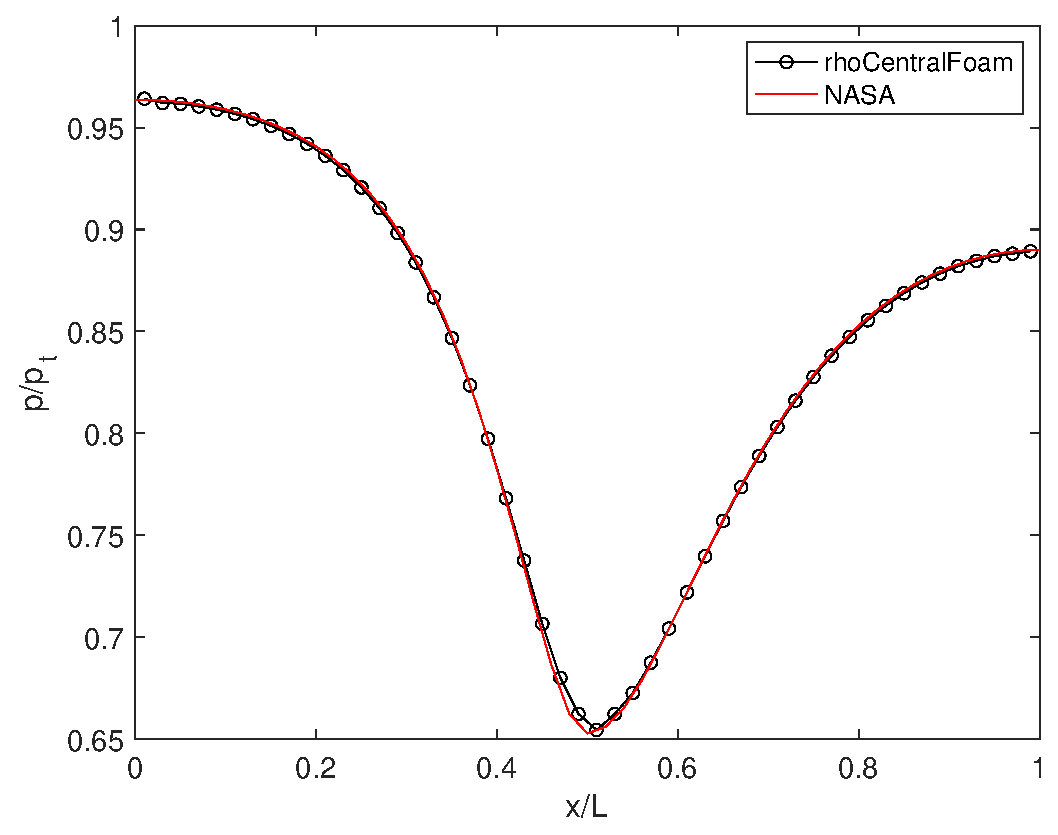
\includegraphics[width=0.475\textwidth]{case1_pratio}
\hfill
\centering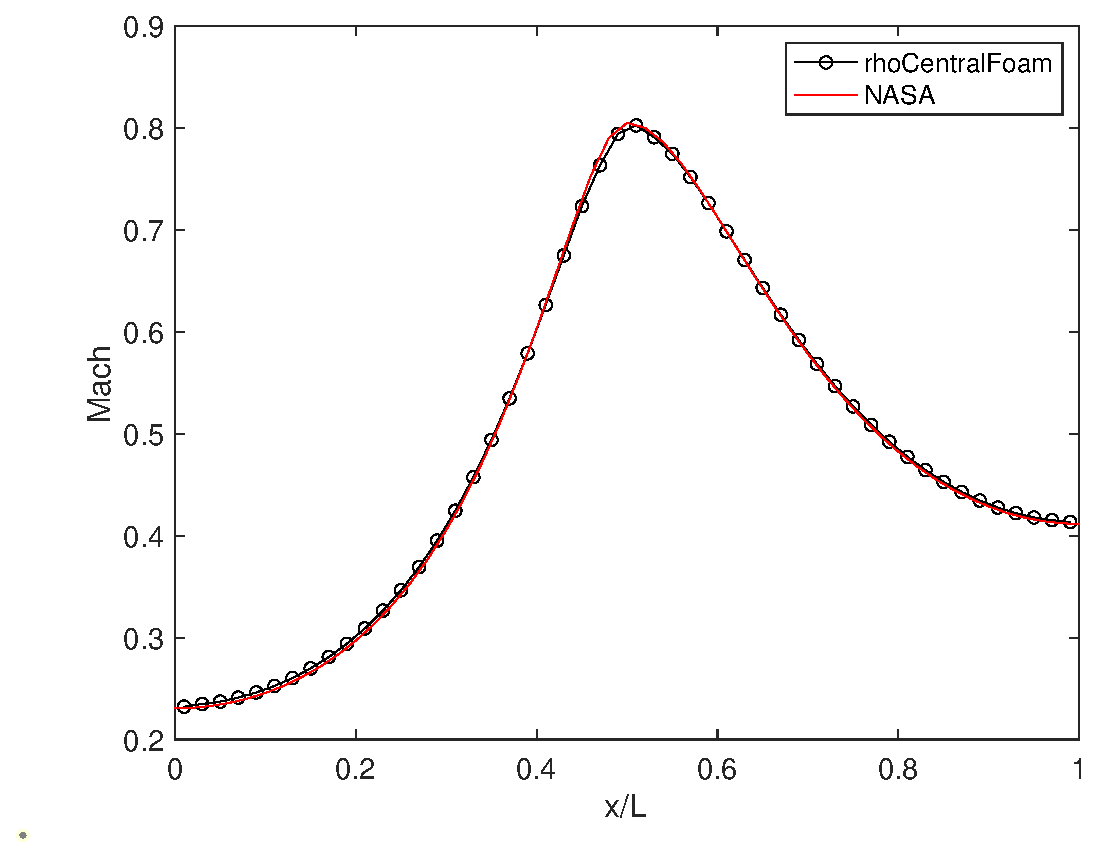
\includegraphics[width=0.475\textwidth]{case1_M}
\caption{Case 1. Pressure ratio  $p/p_t$ (left) and Mach number $M$ (right) along the centerline as
a function of $x/L$ where $L$ is the nozzle length.
The throat is located at $x/L=0.5$}
\label{fig:case1_pics}
\end{figure}

\begin{figure}
\centering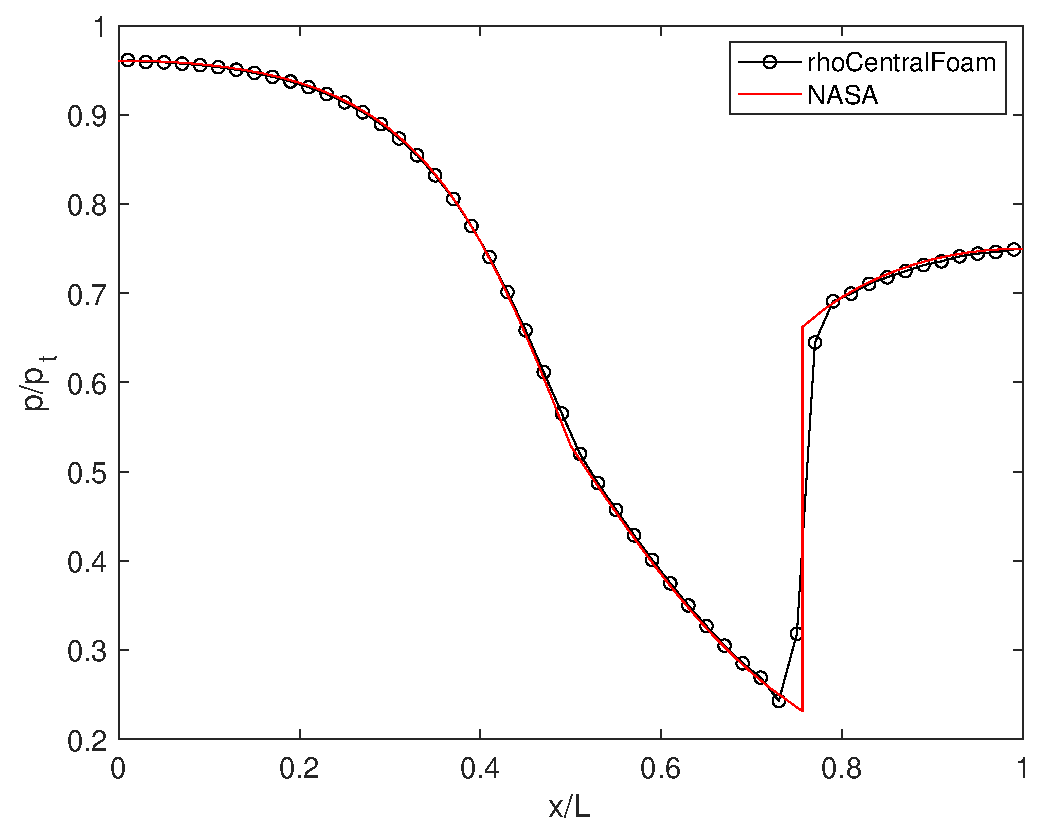
\includegraphics[width=0.475\textwidth]{case2_pratio}
\hfill
\centering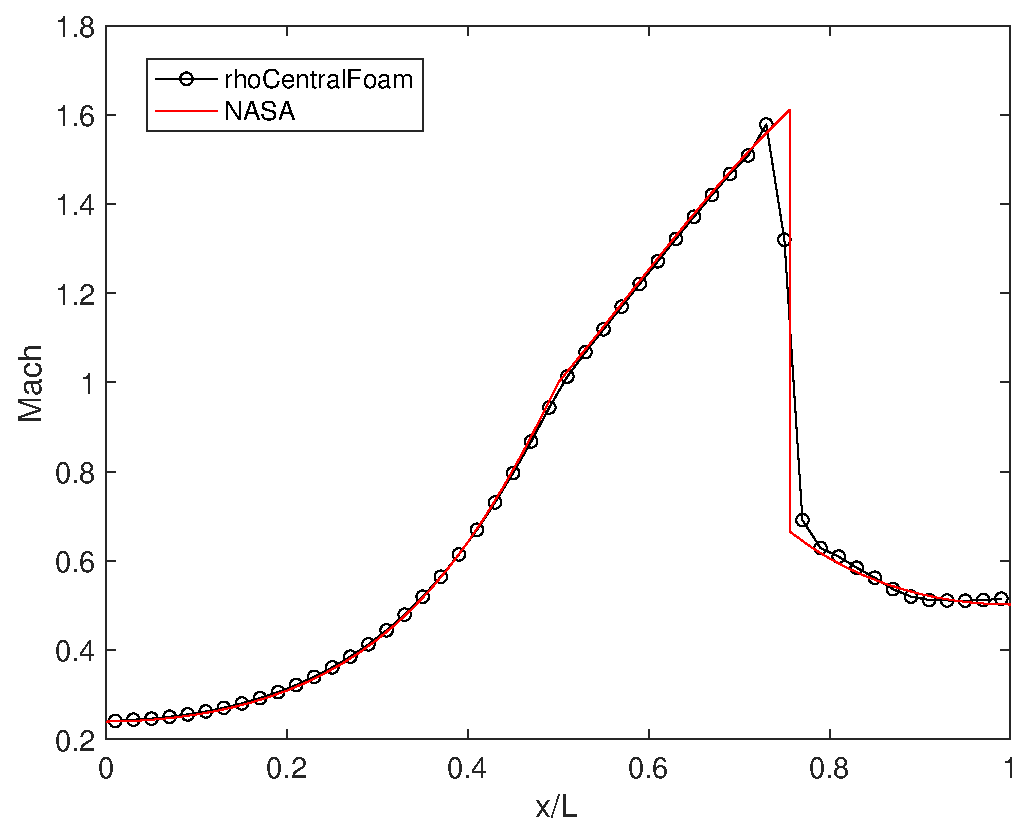
\includegraphics[width=0.475\textwidth]{case2_M}
\caption{Case 2. Pressure ratio  $p/p_t$ (left) and Mach number $M$ (right) along the centerline as
a function of $x/L$ where $L$ is the nozzle length.
The throat is located at $x/L=0.5$}
\label{fig:case1_pics}
\end{figure}

\begin{figure}
\centering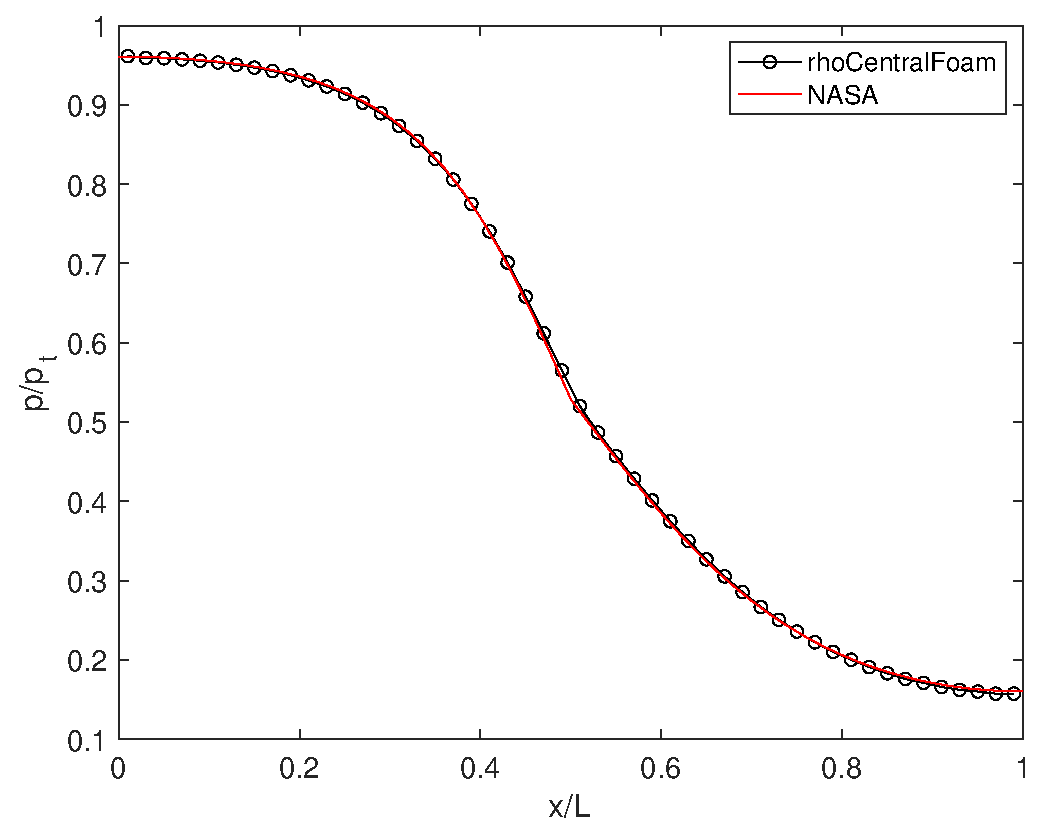
\includegraphics[width=0.475\textwidth]{case3_pratio}
\hfill
\centering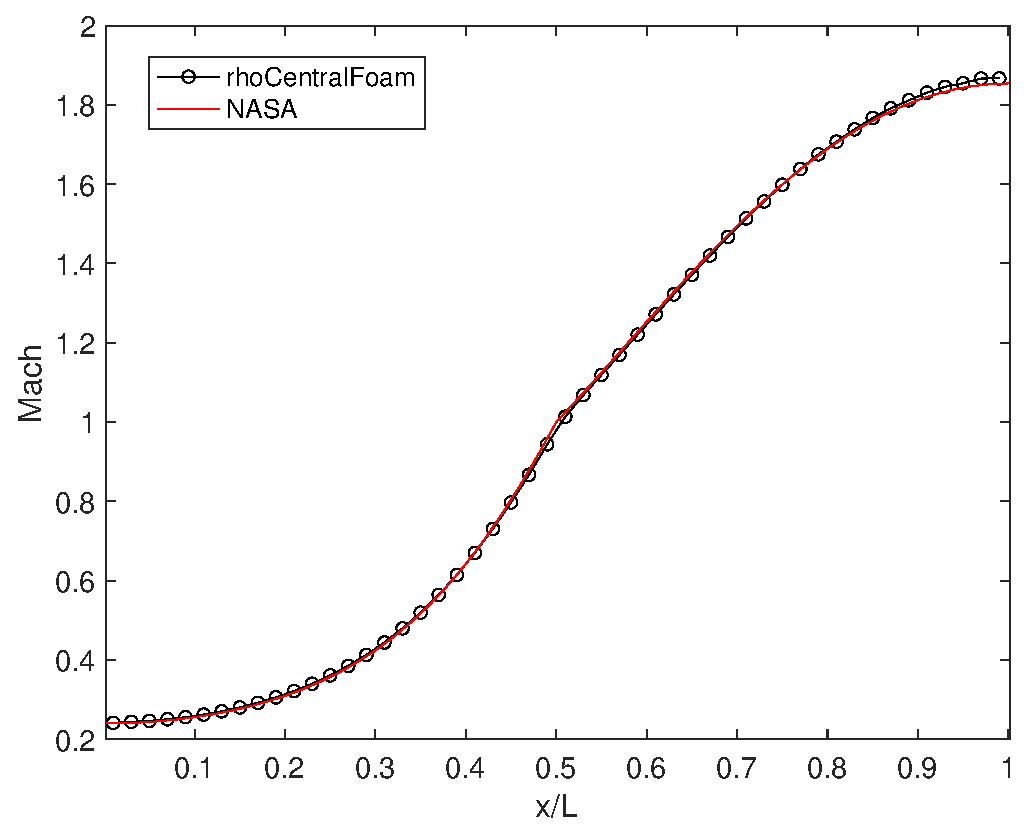
\includegraphics[width=0.475\textwidth]{case3_M}
\caption{Case 3. Pressure ratio  $p/p_t$ (left) and Mach number $M$ (right) along the centerline as
a function of $x/L$ where $L$ is the nozzle length.
The throat is located at $x/L=0.5$}
\label{fig:case1_pics}
\end{figure}



%
\bibliographystyle{unsrtnat}
\bibliography{nozzle}
%
\end{document}
